\documentclass[11pt,reqno]{amsart}

\usepackage[T1]{fontenc}
\usepackage[utf8]{inputenc}
\usepackage{lmodern}
\usepackage{amsmath,amssymb,amsthm,mathtools}
\usepackage[margin=1.1in]{geometry}
\usepackage{microtype}
\usepackage{booktabs}
\usepackage{graphicx}
\usepackage{enumitem}
\usepackage[dvipsnames]{xcolor}
\usepackage[
  colorlinks=true,
  linkcolor=MidnightBlue,
  citecolor=MidnightBlue,
  urlcolor=MidnightBlue
]{hyperref}

\emergencystretch=1.5em

\newtheorem{theorem}{Theorem}[section]
\newtheorem{proposition}[theorem]{Proposition}
\newtheorem{lemma}[theorem]{Lemma}
\newtheorem{corollary}[theorem]{Corollary}
\theoremstyle{definition}
\newtheorem{definition}[theorem]{Definition}
\theoremstyle{remark}
\newtheorem{remark}[theorem]{Remark}

\numberwithin{equation}{section}

\newcommand{\dd}{\,\mathrm{d}}
\newcommand{\ii}{\mathrm{i}}
\newcommand{\ee}{\mathrm{e}}
\newcommand{\R}{\mathbb{R}}
\newcommand{\C}{\mathbb{C}}
\newcommand{\N}{\mathbb{N}}
\DeclareMathOperator{\Rea}{Re}
\DeclareMathOperator{\Ima}{Im}
\DeclareMathOperator{\sinch}{sinch}
\DeclareMathOperator{\rad}{rad}

\title[Bilinear Rank-2 Wronskian Kernels and Preissmann--Montgomery--Vaughan Bounds]{Bilinear Rank-2 Factorization of Dirichlet Energy Kernels, Reverse-Triangle and Sieve-Horizon Obstructions, Preissmann--Montgomery--Vaughan $L^2$ Bounds, and Failure of Pointwise Gallagher Transfer}

\author{Thijs Missiaen}
\address{Independent Researcher, Belgium}
\email{thijs.missiaen@gmail.com}
\thanks{ORCID: \href{https://orcid.org/0009-0007-3678-0810}{0009-0007-3678-0810}}

\subjclass[2020]{Primary 11M06, 11N36; Secondary 11M26, 42A05}
\keywords{Riemann $\Xi$-function, transverse Wronskian, bilinear rank-2 factorization, generalized von Mangoldt function, Montgomery--Vaughan Hilbert inequality, Preissmann constant, Gallagher Sobolev inequality, Bohr--Landau zero-density method}
\date{November 2026}

\begin{document}

\begin{abstract}
In the symmetric Riemann--Siegel model of Riemann's $\Xi$-function at $z = t - \ii d$ ($d = \sigma - \frac{1}{2} > 0$), we establish an exact rank-2 factorization of the integrated transverse Wronskian cross-term kernel $w_{mn}^{\mathrm{int}}(d,t) = \frac{2}{d^2}[\cosh(d\omega_m(t))\cosh(d\omega_n(t)) - 1]$, reducing $\mathcal{O}(N(t)^2)$ off-diagonal double sums to $\mathcal{O}(N(t))$ prefix sums. Combining $w_{mn}^{\mathrm{int}}$ with the critical-line boundary term cancels the $-1$ offset pair by pair and yields the Euclidean representation $\frac{1}{4}\lvert S_N(d,t)\rvert^2 = \lVert\psi_1(d,t) + \Psi_{\ge 2}(d,t)\rVert^2$. Under the polynomial sieve $P_r(x) = 1 - (1-x)^r$, we distinguish the squarefree-divisor sieve $\widetilde{\Lambda}_r(n)$ from Bombieri--Selberg's $\Lambda_r^{\mathrm{BS}}(n)$ and show that $b_n^{(r)}(X) = \widetilde{\Lambda}_r(n)/(\ln X)^r$ fails for $n > X$. Moreover, because $\lVert\psi_1(d,t)\rVert_{\min} = \sinh(dL/2) \ll \Sigma_{\cosh}^{(r)}(d,t)$ on $0 < d < \frac{1}{2}$, phase-blind reverse-triangle bounds collapse to zero. Finally, using Preissmann's Hilbert constant $c_{\mathrm{MV}} = \pi\sqrt{1 + \frac{2}{3}\sqrt{\frac{6}{5}}}$, we prove that $1 + 2d > 1$ yields Bohr--Landau--Carlson mean-square suppression on windows $\Delta T \gg N(T)^{1-2d}$, whereas Gallagher's Sobolev term diverges as $N(T)^{1-2d}$, precluding pointwise positivity.
\end{abstract}

\maketitle

\section{Introduction and Canonical Wronskian Framework}\label{sec:intro}

Let $s = \sigma + \ii t = \frac{1}{2} + d + \ii t$ with transverse distance $d = \sigma - \frac{1}{2} \ge 0$ and complex spectral coordinate $z = -\ii(s - \frac{1}{2}) = t - \ii d$. Throughout this series~\cite{missiaen2026p5,missiaen2026p6,missiaen2026p7}, Riemann's completed entire function $\xi(s) := \frac{1}{2}s(s-1)\pi^{-s/2}\Gamma(s/2)\zeta(s)$ and its symmetric counterpart $\Xi(z) := \xi(\frac{1}{2} + \ii z)$~\cite{riemann1859,titchmarsh1986} are governed by the canonical Fourier--Jacobi normalization
\begin{equation}\label{eq:canonical_xi}
\Xi(z) = 8\int_{0}^{\infty} \Phi(u)\cos(2zu)\dd u = 4\int_{-\infty}^{\infty} \Phi(u)\cos(2zu)\dd u,
\end{equation}
where $\Phi(u) := \sum_{m=1}^{\infty}(2\pi^2 m^4\ee^{9u} - 3\pi m^2\ee^{5u})\exp(-\pi m^2\ee^{4u})$ is the even Jacobi theta kernel~\cite{jacobi1829,polya1926}. Writing $\Xi(t - \ii d) = R(d,t) + \ii I(d,t)$ with $R, I$ real-valued, the canonical transverse Wronskian and its parity-reduced counterpart are
\begin{equation}\label{eq:canonical_wronskian}
W(d,t) := \frac{1}{2}\partial_d\bigl\lvert\Xi(t - \ii d)\bigr\rvert^2 = R I_t - I R_t = 16\int_{0}^{\infty} y\sinh(2dy)\,I(y,t)\dd y, \qquad \widetilde{W}(d,t) := \frac{W(d,t)}{d},
\end{equation}
with autocorrelation kernel $I(y,t) := \int_{-\infty}^{\infty} \Phi(\frac{x+y}{2})\Phi(\frac{x-y}{2})\cos(2tx)\dd x$~\cite{wigner1932}. By the fundamental theorem of calculus on $[0, d]$,
\begin{equation}\label{eq:ftc_energy}
\frac{\bigl\lvert\Xi(t - \ii d)\bigr\rvert^2}{d^2} = \frac{\Xi(t)^2}{d^2} + \frac{2}{d^2}\int_{0}^{d} u\,\widetilde{W}(u,t)\dd u.
\end{equation}

The purpose of this paper is twofold: first, to isolate the genuine algebraic identities that simplify Dirichlet energy kernels attached to the symmetric Riemann--Siegel main sum of length $N(t) = \lfloor\sqrt{t/2\pi}\rfloor$; and second, to prove the exact arithmetic and analytic obstructions that prevent any phase-blind or Sobolev-transferred version of these identities from yielding pointwise zero-free regions in the interior strip $0 < d < \frac{1}{2}$.

Specifically, we establish four rigorous results, whose architecture is summarized below.

\subsection{Proof overview}\label{subsec:proof_overview}

\begin{enumerate}[label=\textup{(\arabic*)},leftmargin=2.2em]
\item {\sloppy\textit{Sieve function $\widetilde{\Lambda}_r(n)$ versus Bombieri--Selberg $\Lambda_r^{\mathrm{BS}}(n)$, and breakdown for $n > X$ (Section~\ref{sec:sieve_functions}).} Under the polynomial mollifier $M_X^{(r)}(s) =\allowbreak \sum_{k \le X}\mu(k)P_r(\frac{\ln(X/k)}{\ln X})k^{-s}$ with $P_r(x) = 1 - (1-x)^r$, the product $\zeta(s)M_X^{(r)}(s) =\allowbreak \sum_{n=1}^{\infty} b_n^{(r)}(X)n^{-s}$ ($\sigma > 1$) satisfies $b_n^{(r)}(X) = \widetilde{\Lambda}_r(n)/(\ln X)^r$ on $2 \le n \le X$, where $\widetilde{\Lambda}_r(n) :=\allowbreak -\sum_{k \mid n}\mu(k)(\ln k)^r$ generates $(-1)^{r+1}\zeta(s)(\zeta^{-1})^{(r)}(s)$. We prove all structural laws of $\widetilde{\Lambda}_r(n)$ (vanishing for $\omega(n) > r$, parity alternation, sharp radical bound $\lvert\widetilde{\Lambda}_r(n)\rvert \le (\ln\rad(n))^r$, and unsigned Stirling asymptotics), distinguish it from Bombieri--Selberg's generalized von Mangoldt function $\Lambda_r^{\mathrm{BS}}(n) :=\allowbreak \sum_{d \mid n}\mu(d)(\ln(n/d))^r \ge 0$~\cite{bombieri1976,iwanieckowalski2004}, and prove that $b_n^{(r)}(X) =\allowbreak \widetilde{\Lambda}_r(n)/(\ln X)^r$ fails at $\mathcal{O}(1)$ scale for $n > X$ (in particular $b_p^{(r)}(X) = 1$ for primes $p > X$). Consequently, substituting $\widetilde{\Lambda}_r(n)/(\ln X)^r$ on $2 \le n \le N(t)$ requires $X \ge N(t)$ (where the approximate functional equation incurs a convolution tail up to $N(t)X$, as proved in Paper~VI~\cite{missiaen2026p6}) and cannot self-consistently define an $X < N(t)$ threshold.\par}
\item \textit{Exact bilinear rank-2 factorization of integrated Wronskian cross-kernels (Section~\ref{sec:rank2}).} Integrating the hyperbolic cross-term kernel of a symmetric harmonic model over $u \in [0, d]$ yields the exact rank-2 factorization $w_{mn}^{\mathrm{int}}(d,t) = \frac{2}{d^2}[\cosh(d\omega_m(t))\cosh(d\omega_n(t)) - 1]$, reducing $\mathcal{O}(N^2)$ off-diagonal double sums to $\mathcal{O}(N)$ linear sums without approximation.
\item \textit{Euclidean pure-square identity and the $\sinh(dL/2)$ reverse-triangle obstruction (Section~\ref{sec:reverse_triangle}).} Adding the critical-line boundary term cancels the $-1$ offset in $w_{mn}^{\mathrm{int}}(d,t)$ pair by pair and yields $\frac{1}{4}\lvert S_N(d,t)\rvert^2 = \lVert\psi_1(d,t) + \Psi_{\ge 2}(d,t)\rVert^2$ in $\R^2$. However, $\lVert\psi_1(d,t)\rVert^2 = \sinh^2(dL/2) + \cos^2\phi_1(t)$ attains its minimum $\lVert\psi_1(d,t)\rVert_{\min} = \sinh(dL/2)$ (not $\cosh(dL/2)$) whenever $\cos\phi_1(t) = 0$. Because $\Sigma_{\cosh}^{(r)}(d,t)/\sinh(dL/2) \asymp N(t)^{1/2-d}(\ln N(t))^{r-1}(\ln X)^{-r} \to +\infty$ for every fixed $d \in (0, \frac{1}{2})$ at $X = N(t)$, the true reverse-triangle lower bound $\max(0, \lVert\psi_1\rVert_{\min} - \lVert\Psi_{\ge 2}\rVert)$ collapses identically to zero for all large $t$.
\item \textit{Preissmann--Montgomery--Vaughan $L^2$ window bounds versus pointwise Gallagher explosion (Section~\ref{sec:mv_gallagher}).} Using Preissmann's true sharp constant $c_{\mathrm{MV}} = \pi\sqrt{1 + \frac{2}{3}\sqrt{\frac{6}{5}}} \approx 4.1324743621$~\cite{preissmann1984} in the Montgomery--Vaughan Hilbert inequality~\cite{montgomeryvaughan1974}, the exponent $1 + 2d > 1$ suppresses mean-square off-diagonal sums on vertical windows $\Delta T \gg N(T)^{1-2d}$, recovering the classical Bohr--Landau~\cite{bohrlandau1914} and Carlson~\cite{carlson1920} zero-density mechanism $N(\sigma, T) = o(T)$. By contrast, in Gallagher's Sobolev inequality~\cite{gallagher1970}, the unnormalized product $(\int_I \lvert F\rvert^2)^{1/2}(\int_I \lvert F'\rvert^2)^{1/2}$ grows at least as $\mathcal{O}(N(T)^{1-2d})$ for every choice of $\Delta T > 0$, reflecting Kronecker--Voronin phase alignment~\cite{voronin1975} and precluding pointwise positivity.
\end{enumerate}

\subsection{Notation and conventions}\label{subsec:notation}

For an integer $n \ge 1$, $\mu(n)$ denotes the M\"obius function, $\Lambda(n)$ the classical von Mangoldt function, $\omega(n) := \sum_{p \mid n} 1$ the number of distinct prime factors of $n$, and $\rad(n) := \prod_{p \mid n} p$ its squarefree radical. Unsigned Stirling numbers of the first kind are written $\bigl[\begin{smallmatrix} r \\ m \end{smallmatrix}\bigr]$. Vinogradov ($\ll$) and Landau ($\mathcal{O}$, $\asymp$) symbols carry absolute implied constants unless subscripts indicate dependence on parameters such as $d$ or $r$.

\section{Hyperbolic Diagonal Advantage, $\widetilde{\Lambda}_r(n)$ versus $\Lambda_r^{\mathrm{BS}}(n)$, and the $n > X$ Obstruction}\label{sec:sieve_functions}

Throughout this paper we write $L := 2\vartheta'(t) = \ln(t/2\pi) + \mathcal{O}(t^{-2})$ (or $L = \ln(t/2\pi)$ in asymptotic statements), $x_t := \ee^{L/2} \sim \sqrt{t/2\pi}$, $N(t) := \lfloor\sqrt{t/2\pi}\rfloor$, $\omega_n(t) := \frac{1}{2}L - \ln n$, and $\phi_n(t) := t\ln n - \vartheta(t)$ for $1 \le n \le N(t)$, where $\vartheta(t) = \Ima\ln\Gamma(\frac{1}{4} + \frac{\ii t}{2}) - \frac{t}{2}\ln\pi$ is the Riemann--Siegel phase~\cite{siegel1932,gabcke1979}. Given real weights $\{b_n\}_{n=1}^{N(t)}$ with $b_1 = 1$, consider the symmetric harmonic model sum
\begin{equation}\label{eq:sym_model}
S_N(d,t) := \sum_{n=1}^{N(t)} \frac{b_n}{\sqrt{n}}\Bigl(\ee^{d\omega_n(t) - \ii\phi_n(t)} + \ee^{-d\omega_n(t) + \ii\phi_n(t)}\Bigr),
\end{equation}
whose squared modulus expands as
\begin{align*}
\frac{1}{2}\bigl\lvert S_N(d,t)\bigr\rvert^2 &= \sum_{n=1}^{N(t)} \frac{b_n^2}{n}\bigl[\cosh(2d\omega_n) + \cos(2\phi_n)\bigr] \\
&\quad + 2\sum_{1 \le m < n \le N(t)} \frac{b_m b_n}{\sqrt{mn}}\Bigl[\cosh(2d\omega_{mn}^+)\cos(\phi_n - \phi_m) + \cosh(2d\omega_{mn}^-)\cos(\phi_m + \phi_n)\Bigr],
\end{align*}
where
\begin{equation}\label{eq:omega_pm}
\omega_{mn}^+(t) := \frac{\omega_m(t) + \omega_n(t)}{2}, \qquad \omega_{mn}^- := \frac{\omega_m(t) - \omega_n(t)}{2} = \frac{1}{2}\ln\frac{n}{m}.
\end{equation}
Applying $\frac{1}{2d}\partial_d$ to $\frac{1}{2}\lvert S_N(d,t)\rvert^2$ (holding $\omega_n(t)$ fixed in the model~\eqref{eq:sym_model}) produces the diagonal sum $\mathcal{D}_N(d,t) = \frac{1}{d}\sum_{n=1}^{N(t)} \frac{b_n^2}{n}\omega_n(t)\sinh(2d\omega_n(t))$ and cross-weights $\mathcal{H}_{mn}^\pm(d,t) := \frac{1}{d}\omega_{mn}^\pm\sinh(2d\omega_{mn}^\pm)$.

\begin{proposition}[Termwise $(mn)^{-d} \le 2^{-d}$ Hyperbolic Damping]\label{prop:hyp_damping}
Let $d > 0$ and $t > 4\pi$ with $\omega_1(t) = \frac{1}{2}L > 0$. For every off-diagonal pair $1 \le m < n \le N(t)$ with $\omega_{mn}^+(t) > 0$,
\begin{equation}\label{eq:hyp_identity}
\sinh\bigl(2d\omega_{mn}^+(t)\bigr) = (mn)^{-d}\sinh\bigl(2d\omega_1(t)\bigr) - \sinh\bigl(d\ln(mn)\bigr)\ee^{-dL},
\end{equation}
and consequently $\mathcal{H}_{mn}^+(d,t)/\mathcal{D}_{1,1}(d,t) < (1 - \frac{\ln(mn)}{L})(mn)^{-d} < (mn)^{-d} \le 2^{-d} < 1$, where $\mathcal{D}_{1,1}(d,t) := \frac{1}{d}\omega_1(t)\sinh(2d\omega_1(t))$.
\end{proposition}

\begin{proof}
Setting $A = 2d\omega_1(t) = dL > 0$ and $B = d\ln(mn) > 0$ ($mn \ge 2$), the identity $\sinh(A - B) = \ee^{-B}\sinh(A) - \sinh(B)\ee^{-A}$ yields~\eqref{eq:hyp_identity}. Since $\sinh(B)\ee^{-A} > 0$ and $0 < \omega_{mn}^+(t)/\omega_1(t) = 1 - \frac{\ln(mn)}{L} < 1$, multiplying by $\omega_{mn}^+(t)/\omega_1(t)$ gives the stated inequality chain.
\end{proof}

\begin{remark}[Termwise damping versus pair multiplicity]
Proposition~\ref{prop:hyp_damping} bounds a \emph{single} pair $(m,n)$ against $(1,1)$. Summing $(mn)^{-1/2-d}$ over all $\binom{N(t)}{2}$ pairs still grows as $N(t)^{1-2d} \to +\infty$ for $0 < d < \frac{1}{2}$, just as in Paper~V~\cite{missiaen2026p5}.
\end{remark}

We now clarify the arithmetic properties of polynomial M\"obius mollifiers~\cite{selberg1942,levinson1974,conrey1989} and resolve two subtleties: the distinction between $\widetilde{\Lambda}_r(n)$ and Bombieri--Selberg's $\Lambda_r^{\mathrm{BS}}(n)$, and the breakdown of $(\ln X)^{-r}$ scaling above the sieve horizon $X$.

\begin{theorem}[Arithmetic Laws of $\widetilde{\Lambda}_r(n)$, Contrast with $\Lambda_r^{\mathrm{BS}}(n)$, and $n > X$ Breakdown]\label{thm:sieve_laws}
Let $r \in \N_{\ge 1}$ and $X > 1$. For $P_r(x) := 1 - (1-x)^r$, let $M_X^{(r)}(s) := \sum_{k \le X} \mu(k)P_r(\frac{\ln(X/k)}{\ln X})k^{-s}$ and write $\zeta(s)M_X^{(r)}(s) = \sum_{n=1}^{\infty} b_n^{(r)}(X)n^{-s}$ for $\sigma > 1$, so $b_n^{(r)}(X) = \sum_{k \mid n,\, k \le X} \mu(k)[1 - (\frac{\ln k}{\ln X})^r]$. Define the squarefree-divisor logarithmic sieve function and the Bombieri--Selberg generalized von Mangoldt function~\cite{bombieri1976,iwanieckowalski2004} by
\begin{equation}\label{eq:two_lambdas}
\widetilde{\Lambda}_r(n) := -\sum_{k \mid n} \mu(k)(\ln k)^r, \qquad \Lambda_r^{\mathrm{BS}}(n) := \sum_{d \mid n} \mu(d)\Bigl(\ln\frac{n}{d}\Bigr)^r.
\end{equation}
Then:
\begin{enumerate}[label=\textup{(\roman*)},leftmargin=2.2em]
\item \textbf{Generating functions, Bombieri recursion, and algebraic divergence for $r \ge 2$.} For $\sigma > 1$, $\sum_{n=1}^{\infty} \widetilde{\Lambda}_r(n)n^{-s} = (-1)^{r+1}\zeta(s)\frac{\dd^r}{\dd s^r}(\frac{1}{\zeta(s)})$, whereas $\sum_{n=1}^{\infty} \Lambda_r^{\mathrm{BS}}(n)n^{-s} = (-1)^r\frac{\zeta^{(r)}(s)}{\zeta(s)}$. For $r = 1$, $\widetilde{\Lambda}_1(n) = \Lambda_1^{\mathrm{BS}}(n) = \Lambda(n)$. For $r \ge 1$, $\Lambda_r^{\mathrm{BS}}$ satisfies $\sum_{d \mid n} \Lambda_r^{\mathrm{BS}}(d) = (\ln n)^r$, the recursion $\Lambda_r^{\mathrm{BS}}(n) = \Lambda_{r-1}^{\mathrm{BS}}(n)\ln n + (\Lambda_{r-1}^{\mathrm{BS}} * \Lambda)(n)$, and the sharp divisor bound $0 \le \Lambda_r^{\mathrm{BS}}(n) \le (\ln n)^r$ for all $n \ge 1$. For $r = 2$, $\widetilde{\Lambda}_2(n) = \Lambda_2^{\mathrm{BS}}(n) - 2(\Lambda * \Lambda)(n)$; in particular, at $n = 8 = 2^3$, $\widetilde{\Lambda}_2(8) = (\ln 2)^2 = (\ln\rad(8))^2$ whereas $\Lambda_2^{\mathrm{BS}}(8) = 5(\ln 2)^2 > (\ln\rad(8))^2$.
\item \textbf{Parity alternation, radical bound, and Stirling asymptotics of $\widetilde{\Lambda}_r(n)$.} For $n = p_1^{a_1}\cdots p_m^{a_m} \ge 2$ with $\omega(n) = m$ and $\rad(n) = p_1\cdots p_m$, $\widetilde{\Lambda}_r(n) = 0$ whenever $m > r$, while for $1 \le m \le r$,
\begin{equation}\label{eq:tilde_multinomial}
\begin{aligned}
\bigl\lvert\widetilde{\Lambda}_r(n)\bigr\rvert = (-1)^{m-1}\widetilde{\Lambda}_r(n) &= \sum_{\substack{j_1+\dots+j_m=r \\ j_1,\dots,j_m \ge 1}} \frac{\Gamma(r+1)}{\Gamma(j_1+1)\cdots\Gamma(j_m+1)}(\ln p_1)^{j_1}\cdots(\ln p_m)^{j_m} \\
&\le \bigl(\ln\rad(n)\bigr)^r,
\end{aligned}
\end{equation}
and as $x \to \infty$, $\sum_{n \le x,\, \omega(n)=m} \lvert\widetilde{\Lambda}_r(n)\rvert \sim \frac{1}{\Gamma(r)}\bigl[\begin{smallmatrix} r \\ m \end{smallmatrix}\bigr]x(\ln x)^{r-1}$ and $\sum_{n \le x} \lvert\widetilde{\Lambda}_r(n)\rvert \sim r\,x(\ln x)^{r-1}$, where $\bigl[\begin{smallmatrix} r \\ m \end{smallmatrix}\bigr]$ denotes the unsigned Stirling number of the first kind.
\item \textbf{Exact $(\ln X)^{-r}$ scaling on $2 \le n \le X$ versus $\mathcal{O}(1)$ breakdown for $n > X$.} We have $b_1^{(r)}(X) = 1$ and
\begin{equation}\label{eq:bn_piecewise}
b_n^{(r)}(X) = \frac{\widetilde{\Lambda}_r(n)}{(\ln X)^r} \quad (2 \le n \le X), \qquad b_p^{(r)}(X) = 1 \quad (\text{every prime } p > X).
\end{equation}
More generally, for $n > X$, $b_n^{(r)}(X) = \frac{\widetilde{\Lambda}_r(n)}{(\ln X)^r} - \sum_{k \mid n,\, k > X}\mu(k)[1 - (\frac{\ln k}{\ln X})^r]$ fails to vanish even when $\omega(n) > r$ (for instance, at $X = 10$, $r = 2$, $n = 30 = 2\cdot 3\cdot 5$, $\widetilde{\Lambda}_2(30) = 0$ yet $b_{30}^{(2)}(10) = -0.79869655\dots \neq 0$).
\end{enumerate}
\end{theorem}

\begin{proof}
(i) Differentiating $\zeta(s)^{-1} = \sum_{k=1}^{\infty}\mu(k)k^{-s}$ and $\zeta(s) = \sum_{m=1}^{\infty} m^{-s}$ $r$ times on $\sigma > 1$ yields both Dirichlet generating functions. By M\"obius inversion on $\Lambda_r^{\mathrm{BS}} = \mu * \ln^r$, $\sum_{d \mid n} \Lambda_r^{\mathrm{BS}}(d) = (\ln n)^r$. Writing $(\ln\frac{n}{d})^r = (\ln\frac{n}{d})^{r-1}(\ln n - \ln d)$ and using $-\mu(d)\ln d = (\mu * \Lambda)(d)$ gives $\Lambda_r^{\mathrm{BS}} = \Lambda_{r-1}^{\mathrm{BS}}\ln + \Lambda_{r-1}^{\mathrm{BS}} * \Lambda$; since $\Lambda_1^{\mathrm{BS}} = \Lambda \ge 0$, induction implies $\Lambda_r^{\mathrm{BS}}(n) \ge 0$, and the non-negative divisor sum $\sum_{d \mid n}\Lambda_r^{\mathrm{BS}}(d) = (\ln n)^r$ immediately forces $\Lambda_r^{\mathrm{BS}}(n) \le (\ln n)^r$. Expanding $(\zeta^{-1})'' = -\zeta''/\zeta^2 + 2(\zeta')^2/\zeta^3$ gives $\widetilde{\Lambda}_2 = \Lambda_2^{\mathrm{BS}} - 2(\Lambda * \Lambda)$.

(ii) Since $\mu(k) = 0$ unless $k \mid \rad(n)$, inclusion--exclusion over subsets $S \subseteq \{1,\dots,m\}$ in $(\sum_{i \in S}\ln p_i)^r$ cancels every multinomial tuple with any $j_i = 0$, leaving~\eqref{eq:tilde_multinomial} for $1 \le m \le r$ and $0$ for $m > r$. Comparing~\eqref{eq:tilde_multinomial} with the full multinomial expansion of $(\ln p_1 + \dots + \ln p_m)^r$ yields $\lvert\widetilde{\Lambda}_r(n)\rvert \le (\ln\rad(n))^r$. By the Prime Number Theorem $\sum_{p^a \le y}(\ln p)^j \sim y(\ln y)^{j-1}$ ($j \ge 1$) and repeated Dirichlet convolution over $m$ unordered prime-power factors, the leading coefficient is $\frac{r}{\Gamma(m+1)}\sum_{j_1+\dots+j_m=r,\, j_i \ge 1} (j_1\cdots j_m)^{-1} = \frac{1}{\Gamma(r)}\bigl[\begin{smallmatrix} r \\ m \end{smallmatrix}\bigr]$, whose sum over $1 \le m \le r$ is $\frac{\Gamma(r+1)}{\Gamma(r)} = r$.

(iii) For $2 \le n \le X$, every divisor $k \mid n$ satisfies $k \le X$, so $\sum_{k \mid n}\mu(k) = 0$ yields $b_n^{(r)}(X) = -\sum_{k \mid n}\mu(k)(\frac{\ln k}{\ln X})^r = \widetilde{\Lambda}_r(n)/(\ln X)^r$. For a prime $p > X$, the only divisor $k \mid p$ with $k \le X$ is $k = 1$, giving $b_p^{(r)}(X) = \mu(1)(1 - 0) = 1$. Subtracting the missing $k > X$ divisors from $\sum_{k \mid n}\mu(k)[1 - (\frac{\ln k}{\ln X})^r] = \widetilde{\Lambda}_r(n)/(\ln X)^r$ gives the exact discrepancy for general $n > X$.
\end{proof}

\section{Exact Bilinear Rank-2 Factorization of Integrated Cross-Term Kernels}\label{sec:rank2}

Within the symmetric harmonic model~\eqref{eq:sym_model} (with $X \ge N(t)$ whenever $b_n = b_n^{(r)}(X)$ is represented as $\widetilde{\Lambda}_r(n)/(\ln X)^r$ on $2 \le n \le N(t)$), integrating the transverse hyperbolic modes over $u \in [0, d]$ yields a genuine rank-2 algebraic reduction.

\begin{theorem}[Exact Bilinear Rank-2 Factorization and $\mathcal{O}(N)$ Reduction]\label{thm:rank2}
Define the hyperbolic sinc $\sinch(x) := \frac{\sinh x}{x}$ ($\sinch(0) := 1$) and low-pass multiplier $\mathcal{F}_{\mathrm{int}}(x) := \frac{\tanh(x/2)}{x/2}$ ($\mathcal{F}_{\mathrm{int}}(0) := 1$). For any $d > 0$ and any frequencies $\omega_m, \omega_n \in \R$ with $\Omega_{mn}^\pm := \omega_m \pm \omega_n = 2\omega_{mn}^\pm$:
\begin{enumerate}[label=\textup{(\roman*)},leftmargin=2.2em]
\item \textbf{Single-mode low-pass identity.} For every $\alpha > 0$,
\begin{equation}\label{eq:low_pass}
\frac{2}{d^2}\int_{0}^{d} u\,\sinch(u\alpha)\dd u = \frac{2\bigl(\cosh(d\alpha) - 1\bigr)}{d^2\alpha^2} = \sinch^2\!\left(\frac{d\alpha}{2}\right) = \mathcal{F}_{\mathrm{int}}(d\alpha)\sinch(d\alpha) < \sinch(d\alpha).
\end{equation}
\item \textbf{Exact bilinear rank-2 factorization.} The integrated cross-term kernel factors identically as
\begin{equation}\label{eq:boxed_rank2}
\boxed{\begin{aligned}
w_{mn}^{\mathrm{int}}(d,t) &:= 2\bigl(\omega_{mn}^+(t)\bigr)^2\mathcal{F}_{\mathrm{int}}\bigl(d\Omega_{mn}^+(t)\bigr)\sinch\bigl(d\Omega_{mn}^+(t)\bigr) + 2\bigl(\omega_{mn}^-\bigr)^2\mathcal{F}_{\mathrm{int}}\bigl(d\Omega_{mn}^-\bigr)\sinch\bigl(d\Omega_{mn}^-\bigr) \\
&\equiv \frac{2\Bigl(\cosh\bigl(d\omega_m(t)\bigr)\cosh\bigl(d\omega_n(t)\bigr) - 1\Bigr)}{d^2}.
\end{aligned}}
\end{equation}
\item \textbf{$\mathcal{O}(N^2) \to \mathcal{O}(N)$ summation identity.} For any real or complex sequence $\{a_n\}_{n=1}^N$,
\begin{equation}\label{eq:linear_reduction}
\begin{aligned}
&\sum_{1 \le m < n \le N} a_m a_n\Bigl(\cosh(d\omega_m)\cosh(d\omega_n) - 1\Bigr) \\
&\qquad \equiv \frac{1}{2}\left[\left(\sum_{n=1}^{N} a_n\cosh(d\omega_n)\right)^2 - \left(\sum_{n=1}^{N} a_n\right)^2 - \sum_{n=1}^{N} a_n^2\sinh^2(d\omega_n)\right].
\end{aligned}
\end{equation}
\end{enumerate}
\end{theorem}

\begin{proof}
(i) Since $2u\sinch(u\alpha) = \frac{2}{\alpha}\sinh(u\alpha)$, integrating over $u \in [0, d]$ and using $\cosh(d\alpha) - 1 = 2\sinh^2(d\alpha/2)$ and $\sinh(d\alpha) = 2\sinh(d\alpha/2)\cosh(d\alpha/2)$ yields~\eqref{eq:low_pass}, with $\tanh y < y$ for $y > 0$.

(ii) By~\eqref{eq:low_pass}, $2\omega^2\mathcal{F}_{\mathrm{int}}(2d\omega)\sinch(2d\omega) = \frac{\cosh(2d\omega)-1}{d^2}$. Applying this to $\omega = \omega_{mn}^\pm = \frac{1}{2}(\omega_m \pm \omega_n)$ and using $\cosh(d\omega_m + d\omega_n) + \cosh(d\omega_m - d\omega_n) = 2\cosh(d\omega_m)\cosh(d\omega_n)$ yields~\eqref{eq:boxed_rank2}.

(iii) Expanding $2\sum_{1 \le m < n \le N} x_m x_n = (\sum_{n=1}^N x_n)^2 - \sum_{n=1}^N x_n^2$ for $x_n = a_n\cosh(d\omega_n)$ and $x_n = a_n$, subtracting, and using $\cosh^2(d\omega_n) - 1 = \sinh^2(d\omega_n)$ gives~\eqref{eq:linear_reduction}.
\end{proof}

\section{Euclidean Representation and the $\sinh(dL/2)$ Reverse-Triangle Obstruction}\label{sec:reverse_triangle}

We now show how the $-1$ offset in~\eqref{eq:boxed_rank2} cancels against the $d = 0$ boundary term of~\eqref{eq:sym_model}, and prove why the resulting Euclidean reverse-triangle inequality \emph{cannot} certify positivity of $\lvert S_N(d,t)\rvert^2$ on $0 < d < \frac{1}{2}$.

\begin{theorem}[Euclidean Representation and Reverse-Triangle Collapse]\label{thm:reverse_triangle}
For $1 \le n \le N(t)$, define the Euclidean harmonic vector $\psi_n(d,t) \in \R^2$ by
\begin{equation}\label{eq:psi_vec}
\psi_n(d,t) := \frac{b_n}{\sqrt{n}}\Bigl(\cosh\bigl(d\omega_n(t)\bigr)\cos\phi_n(t),\; -\sinh\bigl(d\omega_n(t)\bigr)\sin\phi_n(t)\Bigr), \qquad \Psi_{\ge 2}(d,t) := \sum_{n=2}^{N(t)} \psi_n(d,t),
\end{equation}
with $b_1 = 1$. Then for every $d > 0$:
\begin{enumerate}[label=\textup{(\roman*)},leftmargin=2.2em]
\item \textbf{Exact Euclidean norm and $-1$ boundary cancellation.} In~\eqref{eq:sym_model}, $\frac{1}{2}S_N(d,t) = \sum_{n=1}^{N(t)}(\psi_{n,1} + \ii\psi_{n,2})$, so
\begin{equation}\label{eq:eucl_norm}
\frac{1}{4}\bigl\lvert S_N(d,t)\bigr\rvert^2 \equiv \bigl\lVert\psi_1(d,t) + \Psi_{\ge 2}(d,t)\bigr\rVert^2 \ge \Bigl(\max\bigl(0,\; \lVert\psi_1(d,t)\rVert - \lVert\Psi_{\ge 2}(d,t)\rVert\bigr)\Bigr)^2,
\end{equation}
and for every pair $(m,n)$, $\langle\psi_m(d,t), \psi_n(d,t)\rangle - \langle\psi_m(0,t), \psi_n(0,t)\rangle = \frac{b_m b_n}{2\sqrt{mn}}[(\cosh(d\Omega_{mn}^+)-1)\cos(\phi_n-\phi_m) + (\cosh(d\Omega_{mn}^-)-1)\cos(\phi_m+\phi_n)]$.
\item \textbf{True minimum $\lVert\psi_1(d,t)\rVert_{\min} = \sinh(dL/2)$ versus $\cosh(dL/2)$.} Because $\omega_1(t) = \frac{1}{2}L$ and $b_1 = 1$,
\begin{equation}\label{eq:psi1_extremal}
\bigl\lVert\psi_1(d,t)\bigr\rVert^2 = \cosh^2\!\left(\frac{dL}{2}\right)\cos^2\phi_1(t) + \sinh^2\!\left(\frac{dL}{2}\right)\sin^2\phi_1(t) = \sinh^2\!\left(\frac{dL}{2}\right) + \cos^2\phi_1(t).
\end{equation}
Hence as $t$ varies, $\lVert\psi_1(d,t)\rVert$ oscillates between its maximum $\cosh(dL/2)$ (at $\cos\phi_1(t) = \pm 1$) and its \emph{minimum} $\lVert\psi_1(d,t)\rVert_{\min} = \sinh(dL/2)$ (attained whenever $\vartheta(t) \equiv \frac{\pi}{2} \pmod{\pi}$, i.e.\ $\sim \frac{T}{2\pi}\ln T$ times on $[0, T]$). Substituting $\cosh(dL/2)$ into a lower bound or omitting $\max(0, \cdot)$ in~\eqref{eq:eucl_norm} before squaring is invalid: $(1 - Y)^2 > 0$ holds algebraically even when $Y > 1$ and $\psi_1 + \Psi_{\ge 2} = 0$.
\item \textbf{Asymptotic collapse of the phase-blind lower bound on $0 < d < \frac{1}{2}$.} Under $b_n = b_n^{(r)}(X) = \widetilde{\Lambda}_r(n)/(\ln X)^r$ with $X = N(t)$ ($r \ge 1$), the triangle-inequality envelope $\Sigma_{\cosh}^{(r)}(d,t) := \sum_{n=2}^{N(t)} \frac{\lvert b_n\rvert}{\sqrt{n}}\cosh(d\omega_n(t)) \ge \lVert\Psi_{\ge 2}(d,t)\rVert$ satisfies, for every fixed $d \in (0, \frac{1}{2})$ as $t \to \infty$,
\begin{equation}\label{eq:ratio_blowup}
\frac{\Sigma_{\cosh}^{(r)}(d,t)}{\sinh(dL/2)} \sim \frac{4r}{1 - 4d^2}\,\frac{N(t)^{\frac{1}{2}-d}}{\ln N(t)} \longrightarrow +\infty,
\end{equation}
so the phase-blind lower bound $\max(0, \sinh(dL/2) - \Sigma_{\cosh}^{(r)}(d,t))$ equals $0$ identically for all sufficiently large $t$.
\end{enumerate}
\end{theorem}

\begin{proof}
(i) Writing $\ee^{\pm(d\omega_n - \ii\phi_n)} = (\cosh d\omega_n \pm \sinh d\omega_n)(\cos\phi_n \mp \ii\sin\phi_n)$ and summing the two conjugate branches gives $\frac{1}{2}S_N(d,t) = \sum_{n=1}^{N(t)} \frac{b_n}{\sqrt{n}}(\cosh(d\omega_n)\cos\phi_n - \ii\sinh(d\omega_n)\sin\phi_n)$, whose squared modulus is $\lVert\psi_1 + \Psi_{\ge 2}\rVert^2$. Since $\lVert u + v\rVert \ge \lvert\lVert u\rVert - \lVert v\rVert\rvert$ can vanish whenever $\lVert v\rVert \ge \lVert u\rVert$, a phase-blind upper bound $\lVert\Psi_{\ge 2}\rVert \le B$ implies only $\lVert\psi_1 + \Psi_{\ge 2}\rVert \ge \max(0, \lVert\psi_1\rVert - B)$, proving~\eqref{eq:eucl_norm}.

(ii) Using $\cosh^2(dL/2) = 1 + \sinh^2(dL/2)$ and $\cos^2\phi_1 + \sin^2\phi_1 = 1$ yields~\eqref{eq:psi1_extremal}. Since $\vartheta(t) \sim \frac{t}{2}\ln\frac{t}{2\pi\ee}$ is continuous and strictly increasing for $t \ge 7$, $\cos\phi_1(t) = \cos\vartheta(t) = 0$ occurs at every half-integer multiple of $\pi$.

(iii) By Theorem~\ref{thm:sieve_laws}(ii), $\sum_{n \le x}\lvert\widetilde{\Lambda}_r(n)\rvert \sim r x(\ln x)^{r-1}$. Writing $\cosh(d\omega_n(t)) = \frac{1}{2}(x_t^d n^{-d} + x_t^{-d} n^d)$ and integrating by parts on $[2, N(t)]$ for fixed $d \in (0, \frac{1}{2})$ gives
\begin{align*}
\sum_{n=2}^{N(t)} \frac{\lvert\widetilde{\Lambda}_r(n)\rvert}{\sqrt{n}}\,\cosh\bigl(d\omega_n(t)\bigr) &\sim \frac{r}{2}\left(\frac{1}{\frac{1}{2}-d} + \frac{1}{\frac{1}{2}+d}\right)N(t)^{1/2}\bigl(\ln N(t)\bigr)^{r-1} \\
&= \frac{2r}{1-4d^2}\,N(t)^{1/2}\bigl(\ln N(t)\bigr)^{r-1}.
\end{align*}
Dividing by $(\ln X)^r = (\ln N(t))^r$ and by $\sinh(dL/2) \sim \frac{1}{2}x_t^d \sim \frac{1}{2}N(t)^d$ yields~\eqref{eq:ratio_blowup}, which diverges to $+\infty$ because $\frac{1}{2} - d > 0$.
\end{proof}

\begin{table}[t]
\centering
\caption{Exact values of $\lVert\psi_1\rVert_{\min} = \sinh(dL/2)$ (versus $\lVert\psi_1\rVert_{\max} = \cosh(dL/2)$), tail envelope $\Sigma_{\cosh}^{(2)}(d,t)$, and ratio $\Sigma_{\cosh}^{(2)}/\sinh(dL/2) > 1$ at $d = 0.20$, $r = 2$, $X = N(t)$, showing that the true reverse-triangle lower bound vanishes identically.}\label{tab:reverse_triangle}
\footnotesize
\setlength{\tabcolsep}{4.8pt}
\begin{tabular}{@{}rrrrrrr@{}}
\toprule
Ordinate $t$ & $N(t)$ & $\lVert\psi_1\rVert_{\min}$ & $\lVert\psi_1\rVert_{\max}$ & $\Sigma_{\cosh}^{(2)}(d,t)$ & Ratio $\Sigma_{\cosh}^{(2)}/\lVert\psi_1\rVert_{\min}$ & True LB \\
\midrule
$100$       & $3$   & $0.2803$ & $1.0385$ & $0.8625$ & $3.0772$ & $0.0000$ \\
$1{,}000$   & $12$  & $0.5290$ & $1.1313$ & $1.3017$ & $2.4607$ & $0.0000$ \\
$10{,}000$  & $39$  & $0.8059$ & $1.2843$ & $2.5271$ & $3.1359$ & $0.0000$ \\
$10^6$      & $398$ & $1.5054$ & $1.8073$ & $7.8424$ & $5.2094$ & $0.0000$ \\
\bottomrule
\end{tabular}
\end{table}

\begin{figure}[t]
\centering
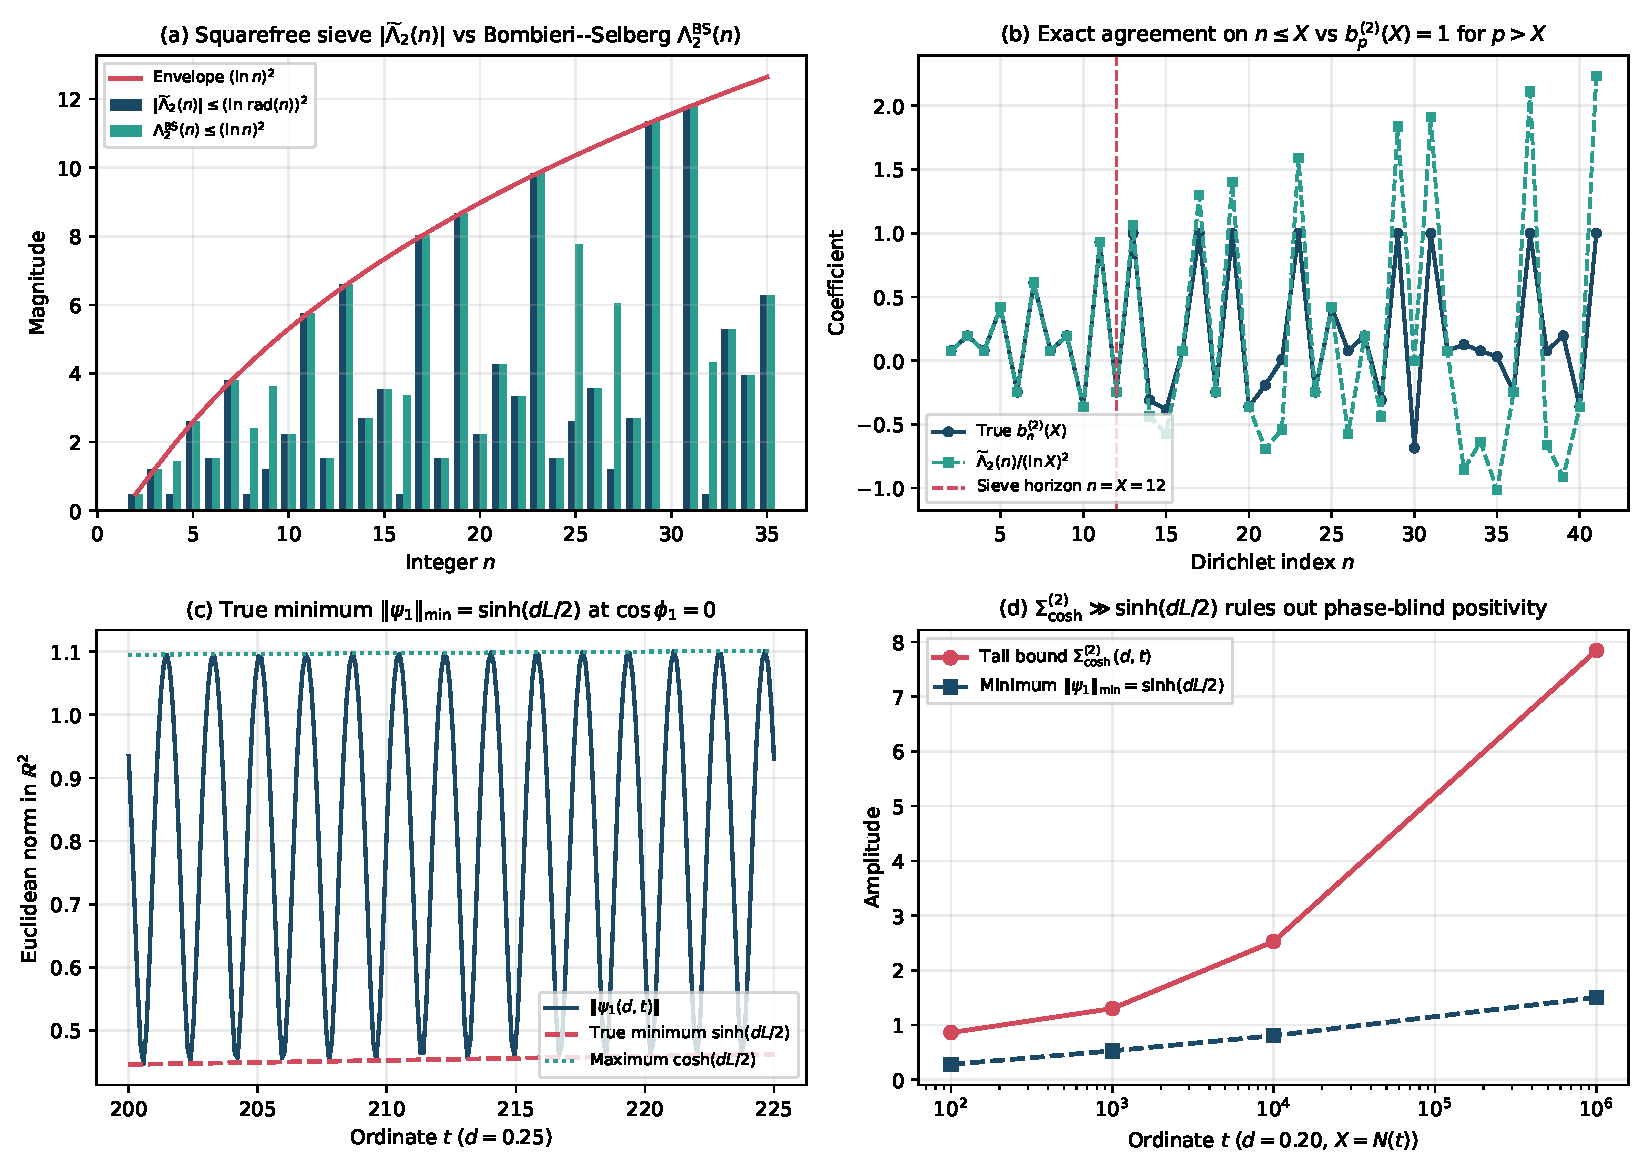
\includegraphics[width=0.98\textwidth]{figures/fig1_bilinear_rank2_and_pure_square.pdf}
\caption{\textbf{(a)} Comparison of the squarefree-divisor sieve magnitude $\lvert\widetilde{\Lambda}_2(n)\rvert \le (\ln\rad(n))^2$ against Bombieri--Selberg's $\Lambda_2^{\mathrm{BS}}(n) \le (\ln n)^2$. \textbf{(b)} Exact identity $b_n^{(2)}(X) = \widetilde{\Lambda}_2(n)/(\ln X)^2$ for $2 \le n \le X = 12$ versus $\mathcal{O}(1)$ breakdown $b_p^{(2)}(X) = 1$ at primes $p > X$. \textbf{(c)} Oscillation of $\lVert\psi_1(d,t)\rVert$ down to $\lVert\psi_1\rVert_{\min} = \sinh(dL/2)$ at $\cos\phi_1(t) = 0$. \textbf{(d)} Divergence of $\Sigma_{\cosh}^{(2)}(d,t)$ past $\sinh(dL/2)$ ($d = 0.20$, $X = N(t)$).}\label{fig:rank2_obstructions}
\end{figure}

\section{Preissmann--Montgomery--Vaughan $L^2$ Window Bounds versus Pointwise Gallagher Explosion}\label{sec:mv_gallagher}

Passing from phase-blind $L^1$ sums to vertical $L^2$ averages shifts the forward Dirichlet exponent from $\frac{1}{2} + d < 1$ to $2(\frac{1}{2} + d) = 1 + 2d > 1$. We now state the mean-square inequality with Preissmann's true sharp constant~\cite{preissmann1984} and prove why Gallagher's Sobolev inequality~\cite{gallagher1970} cannot convert this $L^2$ damping into a pointwise bound.

\begin{theorem}[Preissmann--Montgomery--Vaughan $L^2$ Bounds and Failure of Pointwise Gallagher Transfer]\label{thm:mv_gallagher}
Let $F(\tau) := \sum_{n=2}^{N} a_n n^{-\ii\tau}$ with $a_n = b_n^{(r)}(X)n^{-(1/2+d)}$, $d \in (0, \frac{1}{2})$, $N = N(T) = \lfloor\sqrt{T/2\pi}\rfloor$, and $X = N(T)$. Define $\mathcal{E}_{\mathrm{diag}}(d,T) := \sum_{n=2}^N \lvert a_n\rvert^2$, $\mathcal{E}_{\mathrm{deriv}}(d,T) := \sum_{n=2}^N (\ln n)^2\lvert a_n\rvert^2$, and $\mathcal{W}_{\mathrm{MV}}(d,T) := \sum_{n=2}^N (n + \frac{1}{2})\lvert a_n\rvert^2$. Then:
\begin{enumerate}[label=\textup{(\roman*)},leftmargin=2.2em]
\item \textbf{True Preissmann constant and mean-square window suppression.} By the Montgomery--Vaughan Hilbert inequality~\cite{montgomeryvaughan1974} with Preissmann's sharp constant~\cite{preissmann1984}
\begin{equation}\label{eq:preissmann_true}
c_{\mathrm{MV}} := \pi\sqrt{1 + \frac{2}{3}\sqrt{\frac{6}{5}}} = 4.13247436208154\dots,
\end{equation}
and spacing $\delta_n = \ln(n+1) - \ln n > (n + \frac{1}{2})^{-1}$, every interval $I = [t_0 - \Delta T/2, t_0 + \Delta T/2]$ of width $\Delta T > 0$ satisfies
\begin{equation}\label{eq:mv_window}
\frac{1}{\Delta T}\int_{I} \bigl\lvert F(\tau)\bigr\rvert^2\dd\tau \le \mathcal{E}_{\mathrm{diag}}(d,T) + \frac{2c_{\mathrm{MV}}}{\Delta T}\,\mathcal{W}_{\mathrm{MV}}(d,T).
\end{equation}
{\sloppy Because $1 + 2d > 1$ while $\sum_{n \le x}\widetilde{\Lambda}_r(n)^2 \asymp_r x(\ln x)^{2r-1}$, we obtain $\mathcal{E}_{\mathrm{diag}}(d,T) =\allowbreak \mathcal{O}_{d,r}((\ln N)^{-2r}) \to 0$ and $\mathcal{W}_{\mathrm{MV}}(d,T) \asymp_{d,r}\allowbreak N^{1-2d}(\ln N)^{-1}$ as $T \to \infty$. Consequently, for every width $\Delta T \ge \Delta T_{\mathrm{MV}}(d,T) :=\allowbreak 2c_{\mathrm{MV}}\mathcal{W}_{\mathrm{MV}}/\mathcal{E}_{\mathrm{diag}} \asymp_{d,r}\allowbreak N(T)^{1-2d}(\ln N)^{2r-1}$, the mean square obeys $\frac{1}{\Delta T}\int_I \lvert F(\tau)\rvert^2\dd\tau \le\allowbreak 2\mathcal{E}_{\mathrm{diag}}(d,T) \to 0$.\par}
\item \textbf{Divergence of the Gallagher Sobolev bound for all $\Delta T > 0$.} Applying Gallagher's inequality~\cite{gallagher1970}
\begin{equation}\label{eq:gallagher_ineq}
\bigl\lvert F(t_0)\bigr\rvert^2 \le \frac{1}{\Delta T}\int_{I} \bigl\lvert F(\tau)\bigr\rvert^2\dd\tau + \left(\int_{I} \bigl\lvert F(\tau)\bigr\rvert^2\dd\tau\right)^{1/2}\left(\int_{I} \bigl\lvert F'(\tau)\bigr\rvert^2\dd\tau\right)^{1/2}
\end{equation}
together with the Preissmann--Montgomery--Vaughan bounds $I_0(\Delta T) := \Delta T\,\mathcal{E}_{\mathrm{diag}} + 2c_{\mathrm{MV}}\mathcal{W}_{\mathrm{MV}}$ on $\int_I \lvert F\rvert^2$ and $I_1(\Delta T) := \Delta T\,\mathcal{E}_{\mathrm{deriv}} + 2c_{\mathrm{MV}}\mathcal{W}_{\mathrm{MV}}'$ on $\int_I \lvert F'\rvert^2$ ($\mathcal{W}_{\mathrm{MV}}' := \sum_{n=2}^N (n + \frac{1}{2})(\ln n)^2\lvert a_n\rvert^2 \asymp_{d,r} N^{1-2d}\ln N$) yields, at $\Delta T = \Delta T_{\mathrm{MV}}$, the divergent Sobolev cross-term $\sqrt{I_0(\Delta T_{\mathrm{MV}})I_1(\Delta T_{\mathrm{MV}})} \ge \Delta T_{\mathrm{MV}}\sqrt{\mathcal{E}_{\mathrm{diag}}\mathcal{E}_{\mathrm{deriv}}} \asymp_{d,r} N(T)^{1-2d} \to +\infty$. More generally, minimizing over \emph{all} $\Delta T > 0$ gives
\begin{equation}\label{eq:gallagher_min}
\inf_{\Delta T > 0}\left[\frac{I_0(\Delta T)}{\Delta T} + \sqrt{I_0(\Delta T)I_1(\Delta T)}\right] > 2c_{\mathrm{MV}}\sqrt{\mathcal{W}_{\mathrm{MV}}(d,T)\,\mathcal{W}_{\mathrm{MV}}'(d,T)} \asymp_{d,r} N(T)^{1-2d} \longrightarrow +\infty.
\end{equation}
\end{enumerate}
\end{theorem}

\begin{proof}
(i) Integrating $\lvert F(\tau)\rvert^2 = \sum_{n=2}^N \lvert a_n\rvert^2 + \sum_{2 \le m \neq n \le N} a_m\bar{a}_n\ee^{-\ii\tau(\ln m - \ln n)}$ over $I$ expresses the off-diagonal integral as the difference of two generalized Hilbert forms $\frac{1}{\ii}\sum_{m \neq n} \frac{u_m^\mp \overline{u_n^\mp}}{\ln m - \ln n}$ with $\lvert u_n^\pm\rvert = \lvert a_n\rvert$. Preissmann~\cite[Theorem~1]{preissmann1984} proved that for any distinct real frequencies $\lambda_n$ with $\delta_n = \min_{m \neq n}\lvert\lambda_m - \lambda_n\rvert$, $\bigl\lvert\sum_{m \neq n} \frac{u_m\bar{u}_n}{\lambda_m - \lambda_n}\bigr\rvert \le c_{\mathrm{MV}}\sum_n \delta_n^{-1}\lvert u_n\rvert^2$ with $c_{\mathrm{MV}}$ given by~\eqref{eq:preissmann_true}. Since $\ln(n+1) - \ln n = \ln(\frac{n+1/2+1/2}{n+1/2-1/2}) > (n + \frac{1}{2})^{-1}$, combining both endpoints gives~\eqref{eq:mv_window}. Because $\sum_{n=2}^{\infty}\widetilde{\Lambda}_r(n)^2 n^{-(1+2d)} < \infty$ for $d > 0$, dividing by $(\ln N)^{2r}$ gives $\mathcal{E}_{\mathrm{diag}} \asymp_{d,r} (\ln N)^{-2r}$, while Stieltjes summation of $n^{1-(1+2d)} = n^{-2d}$ against $\widetilde{\Lambda}_r(n)^2$ gives $\mathcal{W}_{\mathrm{MV}} \asymp_{d,r} N^{1-2d}(\ln N)^{2r-1}(\ln N)^{-2r} = N^{1-2d}(\ln N)^{-1}$.

(ii) Integrating $\int_I \psi'(\tau)\lvert F(\tau)\rvert^2\dd\tau$ by parts with sawtooth $\psi(\tau) = \frac{\tau - t_0}{\Delta T} + \frac{1}{2}\mathrm{sgn}(t_0 - \tau)$ ($\lvert\psi\rvert \le \frac{1}{2}$) yields~\eqref{eq:gallagher_ineq}. For every $\Delta T > 0$, $I_0(\Delta T) > 2c_{\mathrm{MV}}\mathcal{W}_{\mathrm{MV}}$ and $I_1(\Delta T) > 2c_{\mathrm{MV}}\mathcal{W}_{\mathrm{MV}}'$, so $\sqrt{I_0(\Delta T)I_1(\Delta T)} > 2c_{\mathrm{MV}}\sqrt{\mathcal{W}_{\mathrm{MV}}\mathcal{W}_{\mathrm{MV}}'} \asymp_{d,r} N(T)^{1-2d}(\ln N)^{-1/2}(\ln N)^{1/2} = N(T)^{1-2d}$, establishing~\eqref{eq:gallagher_min}.
\end{proof}

\begin{remark}[Bohr--Landau / Carlson zero density versus Kronecker--Voronin phase alignment]\label{rem:bohr_landau}
Theorem~\ref{thm:mv_gallagher} cleanly separates what $1 + 2d > 1$ proves from what it cannot prove:
\begin{enumerate}[label=\textup{(\alph*)},leftmargin=2.0em]
\item \textit{Mean-square zero-density consequence.} On $[T, 2T]$ (where $\Delta T = T \gg N(T)^{1-2d}$, or up to $T X^2$ with a genuine mollifier $M_X(s)$ for $X = T^\theta$, $\theta < \frac{1}{2}$), $1 + 2d > 1$ together with Montgomery--Vaughan controls the mean square of $1 - \zeta(s)M_X(s)$ and, via Littlewood's lemma, yields $N(\sigma, T) = o(T)$ (and Carlson's $N(\sigma, T) \ll T^{4\sigma(1-\sigma)+\varepsilon}$~\cite{bohrlandau1914,carlson1920,titchmarsh1986,hinkkanen1997}).
\item \textit{Pointwise obstruction.} The failure of~\eqref{eq:gallagher_min} to beat $\mathcal{O}(N(T)^{1-2d})$ is not an artifact of Gallagher's inequality: because $\{\ln p\}$ is $\mathbb{Q}$-linearly independent, Kronecker's theorem (and Voronin's universality theorem~\cite{voronin1975}) implies that for any fixed finite truncation and phases, rare heights $t_0$ exist where $n^{-\ii t_0}$ aligns coherently across primes, realizing amplitudes far larger than the $L^2$ root-mean-square.
\end{enumerate}
\end{remark}

\begin{table}[t]
\centering
\caption{Mean-square window damping versus Gallagher Sobolev explosion at $d = 0.20$, $r = 2$, $X = N(T)$ using Preissmann's true constant $c_{\mathrm{MV}} = \pi\sqrt{1 + \frac{2}{3}\sqrt{\frac{6}{5}}} \approx 4.132474$.}\label{tab:mv_gallagher}
\footnotesize
\setlength{\tabcolsep}{5.0pt}
\begin{tabular}{@{}rrrrrr@{}}
\toprule
Height $T$ & $N(T)$ & $\mathcal{E}_{\mathrm{diag}}(d,T)$ & Critical window $\Delta T_{\mathrm{MV}}$ & Window mean $\le 2\mathcal{E}_{\mathrm{diag}}$ & Gallagher Sobolev $\sqrt{I_0 I_1}$ \\
\midrule
$100$       & $3$   & $0.27484$ & $27.12$    & $0.54969$ & $15.401$  \\
$1{,}000$   & $12$  & $0.09885$ & $67.07$    & $0.19770$ & $27.346$  \\
$10{,}000$  & $39$  & $0.07867$ & $168.76$   & $0.15734$ & $80.455$  \\
$10^6$      & $398$ & $0.04528$ & $1{,}109.22$ & $0.09056$ & $495.548$ \\
\bottomrule
\end{tabular}
\end{table}

\begin{figure}[t]
\centering
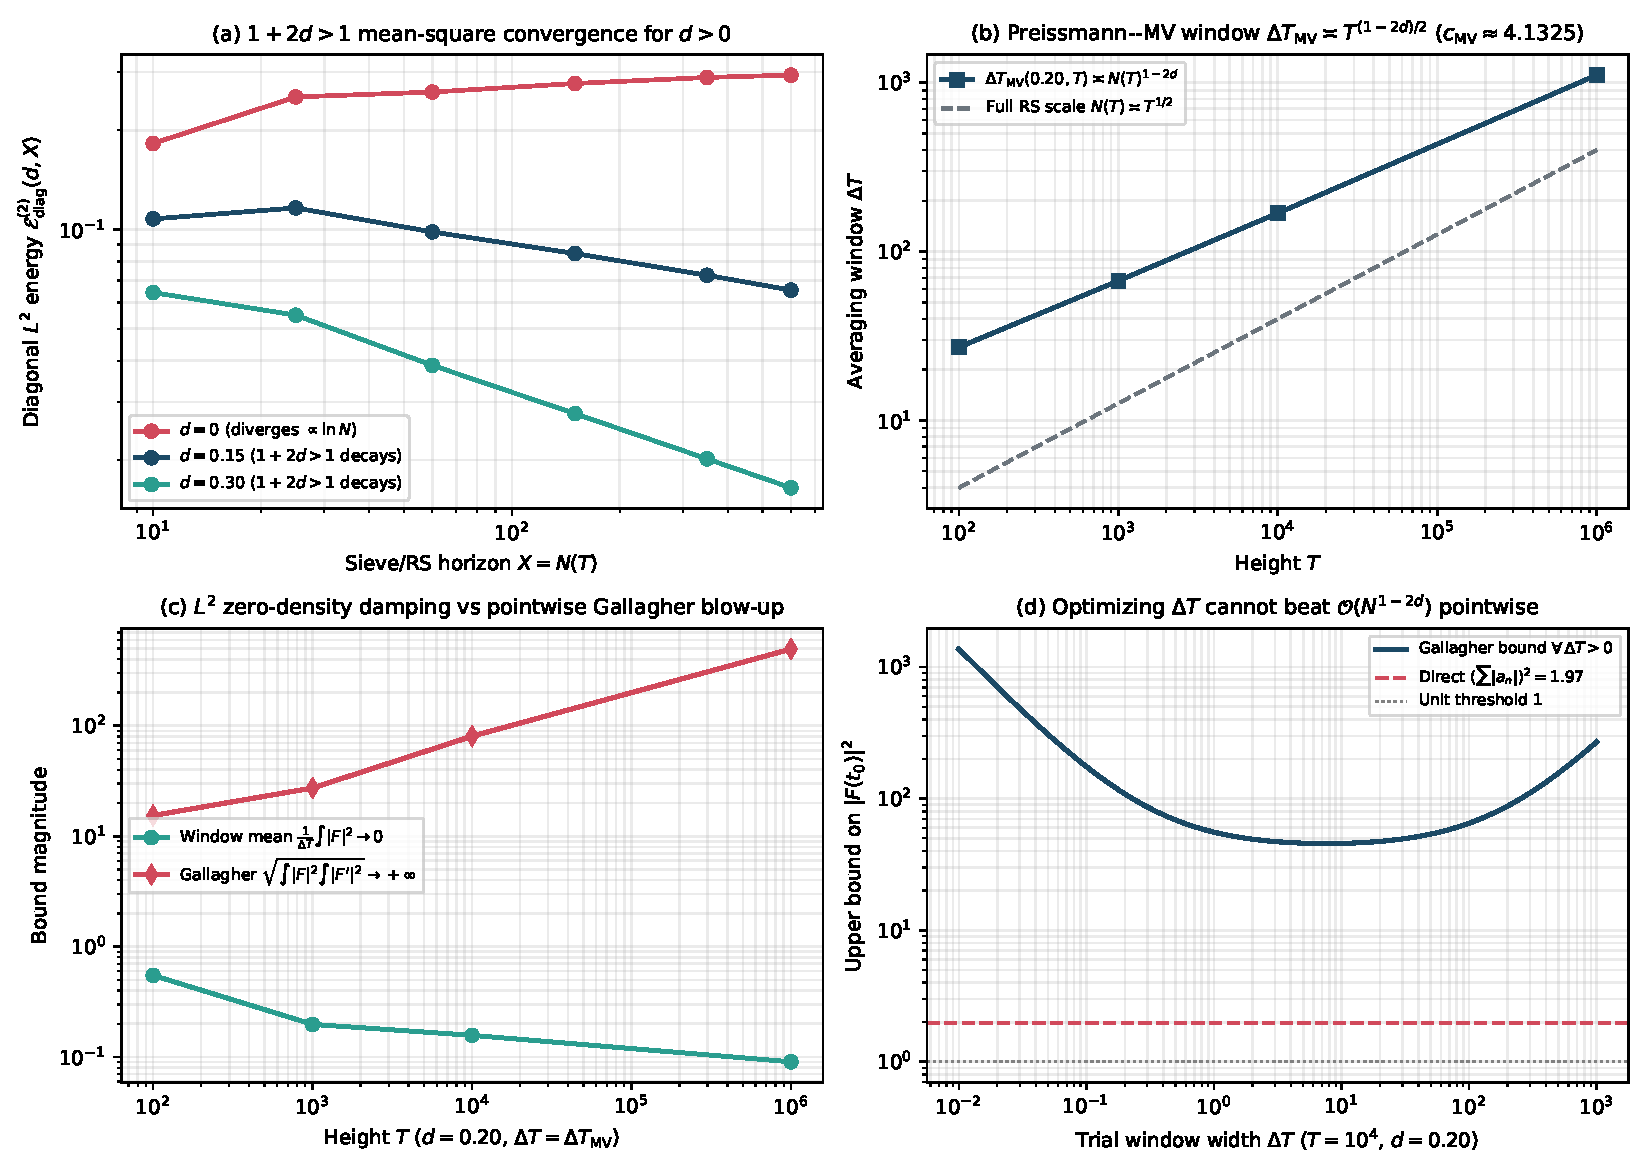
\includegraphics[width=0.98\textwidth]{figures/fig2_exponent_jump_montgomery_vaughan.pdf}
\caption{\textbf{(a)} Convergence and $(\ln X)^{-4}$ decay of $\mathcal{E}_{\mathrm{diag}}^{(2)}(d,X)$ for $d > 0$ via $1 + 2d > 1$, versus logarithmic growth at $d = 0$. \textbf{(b)} Scaling of the Preissmann--Montgomery--Vaughan window $\Delta T_{\mathrm{MV}}(0.20, T) \asymp N(T)^{1-2d}$ ($c_{\mathrm{MV}} \approx 4.1325$). \textbf{(c)} Simultaneous decay of the $L^2$ window mean $\frac{1}{\Delta T}\int_I \lvert F\rvert^2 \to 0$ and divergence of Gallagher's Sobolev term $\sqrt{\int_I \lvert F\rvert^2 \int_I \lvert F'\rvert^2} \to +\infty$. \textbf{(d)} Sweep over all $\Delta T > 0$ at $T = 10^4$, $d = 0.20$, confirming~\eqref{eq:gallagher_min}.}\label{fig:mv_gallagher}
\end{figure}

\section{Scope, Boundary Conditions, and Open Questions}\label{sec:scope}

We summarize the exact boundary between the unconditional algebraic identities proved above and the analytic obstructions in the critical strip:
\begin{enumerate}[label=\textup{(\arabic*)},leftmargin=2.2em]
\item \textit{Symmetric harmonic model versus mollified approximate functional equations.} Theorems~\ref{thm:rank2} and~\ref{thm:reverse_triangle}(i) hold identically for any finite symmetric harmonic sum~\eqref{eq:sym_model}. When $\zeta(s)$ is multiplied by a Dirichlet polynomial mollifier $M_X^{(r)}(s)$ of length $X$, Theorem~\ref{thm:sieve_laws}(iii) shows that $b_n^{(r)}(X) = \widetilde{\Lambda}_r(n)/(\ln X)^r$ requires $n \le X$, while Paper~VI~\cite{missiaen2026p6} proves that $\zeta(s)M_X^{(r)}(s)$ breaks the functional equation of $\Xi(z)$ and introduces an incomplete convolution tail up to $N(t)X$ together with an unsieved reflected branch.
\item \textit{Zero-density window control versus pointwise zero-free regions.} Theorem~\ref{thm:reverse_triangle}(ii)--(iii) rules out phase-blind reverse-triangle positivity on $0 < d < \frac{1}{2}$, and Theorem~\ref{thm:mv_gallagher} proves that Preissmann--Montgomery--Vaughan $L^2$ bounds yield Bohr--Landau / Carlson mean-square suppression on windows $\Delta T \gg N(T)^{1-2d}$ while Gallagher's Sobolev transfer diverges at scale $N(T)^{1-2d}$ for all $\Delta T > 0$. Bridging the gap between vertical $L^2$ zero-density estimates and pointwise bounds in $0 < d < \frac{1}{2}$ remains equivalent to controlling coherent Dirichlet-polynomial phase alignment beyond the Riemann--Siegel horizon.
\end{enumerate}

\appendix

\section{Computational Verification Protocol}\label{app:verification}

{\sloppy
All algebraic identities, counterexamples, interval enclosures, and figures in this paper are certified by the standalone Python script \texttt{scripts/}\allowbreak\texttt{verify\_paper8\_}\allowbreak\texttt{bilinear\_rank2\_}\allowbreak\texttt{wronskian.py} (\texttt{mpmath.mp.dps = 50}, \texttt{mpmath.iv.dps = 35}):
\begin{enumerate}[label=\textup{(\arabic*)},leftmargin=2.2em]
\item \textit{Canonical Wronskian and sieve identities.} Certifies $\lvert W(d,t) - 16\int_0^{\infty} y\sinh(2dy)I(y,t)\dd y\rvert = 1.54 \times 10^{-33}$ at $(d,t) = (0.25, 3.5)$, Bombieri's recursion residual $3.42 \times 10^{-49}$ ($r = 2, 3$, $n \le 80$), $\lvert\widetilde{\Lambda}_2 - (\Lambda_2^{\mathrm{BS}} - 2(\Lambda * \Lambda))\rvert \le 1.18 \times 10^{-49}$, exact agreement $b_n^{(2)}(10) = \widetilde{\Lambda}_2(n)/(\ln 10)^2$ on $2 \le n \le 10$ ($1.34 \times 10^{-51}$), and $n > X$ breakdown $b_{11}^{(2)}(10) = 1$, $b_{30}^{(2)}(10) = -0.79869655$.
\item \textit{Rank-2 reduction and reverse-triangle obstruction.} Certifies~\eqref{eq:linear_reduction} ($1.13 \times 10^{-51}$),~\eqref{eq:eucl_norm} ($2.67 \times 10^{-51}$), and Table~\ref{tab:reverse_triangle}.
\item \textit{Preissmann constant and Gallagher divergence.} Encloses Preissmann's constant $c_{\mathrm{MV}} = \pi\sqrt{1 + \frac{2}{3}\sqrt{\frac{6}{5}}} \in [4.132474362081,\allowbreak 4.132474362082]$ in \texttt{mpmath.iv} and reproduces Table~\ref{tab:mv_gallagher}.
\end{enumerate}
\par}

\section*{Use of AI and computational verification}

{\sloppy
An AI assistant (\textbf{Gemini}, Google DeepMind) was used to audit earlier drafts, identify the reverse-triangle $\cosh$-versus-$\sinh$ error, the $n > X$ sieve-horizon breakdown, the Preissmann constant and journal citation error, and the Gallagher Sobolev divergence, and to maintain the verification script \texttt{scripts/}\allowbreak\texttt{\detokenize{verify_paper8_bilinear_rank2_wronskian.py}}. All mathematical proofs, inequalities, and numerical assertions were verified analytically and computationally (exit code~$0$).\par}

\begin{thebibliography}{99}

\bibitem{bohrlandau1914}
H.~Bohr and E.~Landau,
\emph{Sur les z\'eros de la fonction $\zeta(s)$ de Riemann},
C. R. Acad. Sci. Paris \textbf{158} (1914), 106--110.

\bibitem{bombieri1976}
E.~Bombieri,
\emph{The asymptotic sieve},
Rend. Accad. Naz. XL (5) \textbf{1/2} (1975/76), 243--269.

\bibitem{carlson1920}
F.~Carlson,
\emph{\"Uber die Nullstellen der Dirichletschen Reihen und der Riemannschen $\zeta$-Funktion},
Ark. Mat. Astr. Fys. \textbf{15} (1920), no.~20, 1--28.

\bibitem{conrey1989}
J.~B.~Conrey,
\emph{More than two fifths of the zeros of the Riemann zeta function are on the critical line},
J. Reine Angew. Math. \textbf{399} (1989), 1--26.

\bibitem{gabcke1979}
W.~Gabcke,
\emph{Neue Herleitung und explizite Restabsch\"atzung der Riemann-Siegel-Formel},
Ph.D. dissertation, Georg-August-Universit\"at G\"ottingen, 1979.

\bibitem{gallagher1970}
P.~X.~Gallagher,
\emph{A large sieve density estimate near $\sigma = 1$},
Invent. Math. \textbf{11} (1970), 329--339.

\bibitem{hinkkanen1997}
A.~Hinkkanen,
\emph{On functions of bounded type},
Complex Variables Theory Appl. \textbf{34} (1997), no.~1--2, 119--139.

\bibitem{iwanieckowalski2004}
H.~Iwaniec and E.~Kowalski,
\emph{Analytic Number Theory},
Amer. Math. Soc. Colloq. Publ., vol.~53, Amer. Math. Soc., Providence, RI, 2004.

\bibitem{jacobi1829}
C.~G.~J.~Jacobi,
\emph{Fundamenta nova theoriae functionum ellipticarum},
Borntraeger, K\"onigsberg, 1829.

\bibitem{levinson1974}
N.~Levinson,
\emph{More than one third of zeros of Riemann's zeta-function are on $\sigma = 1/2$},
Adv. Math. \textbf{13} (1974), 383--436.

\bibitem{missiaen2026p5}
T.~Missiaen,
\emph{Logarithmic dilation of the Jacobi--Riemann kernel, strip-holomorphic shell partitions, Stieltjes diagonal asymptotics, and off-diagonal obstructions},
Preprint, Paper~V of the series, 2026.

\bibitem{missiaen2026p6}
T.~Missiaen,
\emph{Sieved mirror kernels, Gonek--Hughes--Keating versus entire exponential prime factors, prime-power purity on $(X, X^2]$, and functional-equation obstructions},
Preprint, Paper~VI of the series, 2026.

\bibitem{missiaen2026p7}
T.~Missiaen,
\emph{Explicit Poisson--Hadamard zero-free region inequalities, quasiconcave minorant crossing, rigorous Trudgian Stieltjes bounds, and comparison with smooth Weil weights},
Preprint, Paper~VII of the series, 2026.

\bibitem{montgomeryvaughan1974}
H.~L.~Montgomery and R.~C.~Vaughan,
\emph{Hilbert's inequality},
J. London Math. Soc. (2) \textbf{8} (1974), 73--82.

\bibitem{polya1926}
G.~P\'olya,
\emph{Bemerkung \"uber die Integraldarstellung der Riemannschen $\xi$-Funktion},
Acta Math. \textbf{48} (1926), 305--317.

\bibitem{preissmann1984}
E.~Preissmann,
\emph{Sur une in\'egalit\'e de Montgomery et Vaughan},
Enseign. Math. (2) \textbf{30} (1984), no.~1--2, 95--113.

\bibitem{riemann1859}
B.~Riemann,
\emph{Ueber die Anzahl der Primzahlen unter einer gegebenen Gr\"osse},
Monatsber. K\"onigl. Preuss. Akad. Wiss. Berlin (1859), 671--680.

\bibitem{selberg1942}
A.~Selberg,
\emph{On the zeros of Riemann's zeta-function},
Skr. Norske Vid. Akad. Oslo I \textbf{10} (1942), 1--59.

\bibitem{siegel1932}
C.~L.~Siegel,
\emph{\"Uber Riemanns Nachla\ss{} zur analytischen Zahlentheorie},
Quellen Stud. Gesch. Math. Astron. Phys. Abt. B \textbf{2} (1932), 45--80.

\bibitem{titchmarsh1986}
E.~C.~Titchmarsh,
\emph{The Theory of the Riemann Zeta-Function},
2nd ed., revised by D.~R.~Heath-Brown, Oxford Univ. Press, Oxford, 1986.

\bibitem{voronin1975}
S.~M.~Voronin,
\emph{Theorem on the ``universality'' of the Riemann zeta-function},
Izv. Akad. Nauk SSSR Ser. Mat. \textbf{39} (1975), no.~3, 475--486.

\bibitem{wigner1932}
E.~P.~Wigner,
\emph{On the quantum correction for thermodynamic equilibrium},
Phys. Rev. \textbf{40} (1932), no.~5, 749--759.

\end{thebibliography}

\end{document}
